\documentclass[12pt]{article}
\usepackage[utf8]{inputenc}

\title{Sprawozdanie\\z projektu indywidualnego\\,,Analiza Grafów z CUDAC''}
\author{Daniel Sporysz}
\date{06.06.2019}

\usepackage{natbib}
\usepackage{graphicx}
\usepackage{polski}
\usepackage{indentfirst}
\usepackage{geometry}

\usepackage{listings} % Required for inserting code snippets

\begin{document}

\makeatletter
\newcommand{\linia}{\rule{\linewidth}{0.4mm}}
\renewcommand{\maketitle}{\begin{titlepage}
    \begin{center}\LARGE
    Politechnika Warszawska\\Wydział Elektryczny
    \end{center}
    \vspace{4cm}
    \noindent
    \begin{center}
      \LARGE \textsc{\@title}
         \end{center}
    \vspace{4cm}
    \begin{flushright}
    \begin{minipage}{5cm}
    \textit{Autor:}\\
    \normalsize \textsc{\@author} \par
    \end{minipage}
     \end{flushright}
    \vspace*{\stretch{6}}
    \begin{center}
    \vspace*{\fill}
    \@date
    \end{center}
  \end{titlepage}%
}
\makeatother

\maketitle
\newpage

\tableofcontents
\newpage

\section{Wprowadzenie}
Postęp technologiczny procesorów mocno zahamował, co objawia się małym przyrostem wydajności z generacji na generację. Podczas gdy zapotrzebowanie na moc obliczeniową rosnie. Rozwiązaniem jest, przynajmniej częsci problemów, zrównoleglanie pracy. Olbrzymi potencjał obliczeń równoległbych tkwi w kartach graficznych, a bilbioteka CUDAC umożliwa na jego wykorzystanie.
Celem projektu jest zapoznanie się z tą technologią, a tematem ćwiczeniowym jest analiza grafów skierowanych w celu poszukiwania cykli.
Wybrany algorytm poszykiwania elementów silnie związanych w grafie, został zaimplementowany w dwóch wersjach - tylko na procesorze CPU i druga z wykorzystaniem karty graficznej.

\section{Koncept}
Do realizacji zadania, postanowiłem zaimplementować i zrównoleglić algorytm Depth-first Search (DFS). W wersji na kartę graficzną, każdy pojedyńczy wątek zajmuje się analizą drogi od jednego węzła grafu - im więcej węzłow w grafie, tym więcej wątków zostanie uruchomionych.

\section{Analiza wyników z implementacji}
\subsection{Metodyka testowania}
Do porównania wersji na CPU do wersji na GPU, wykorzystane zostały grafy, gdzie każdy węzeł miał połączenie z pozostałymi (relacja każdy z każdym), tak aby zmierzyć wydajność w przypadkach najmniej korzystnych.

Programy uruchamiane były na systeme Windows 10 Pro, pracujący na sprzęcie:
\begin{enumerate}
    \item CPU: AMD Ryzen 1600
    \item RAM: 8GB DualChannel 2933Mhz cl15
    \item GPU: Nvidia GTX 950
\end{enumerate}

\subsection{Wyniki testów}

\begin{center}
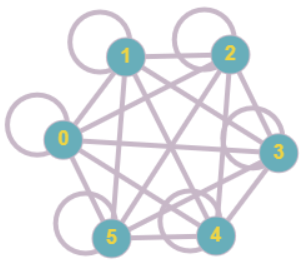
\includegraphics{graph.png}
\end{center}

Z racji, że dane wejściowe generowały olbrzymią ilość cykli, a te przechowywane były w obiektach std::vector, niemożliwe było przetestowanie wydajności programu na grafach o ilości węzłow większej niż 10. Wyniki zapełniamy pamięć RAM.

Niestety kolejne ograniczenie dotyczy wersji na GPU. Limitem górnym okazało się 8 wezłów w grafie. Powyżej tej liczby, karta graficzna nie pozwalała zaalokować pamięci dla dużej ilości cykli.

\begin{table}[ht]
    \centering
    \begin{tabular}{|c|c|c|c|}
    \hline
    Wymiary grafu & Czas analizy na CPU & Czas analizy na GPU & Liczba cykli w grafie\\
    \hline
    \hline
    10 & 8936 ms & - & 9864100\\
    \hline
    9 & 846 ms & - & 986409\\
    \hline
    8 & 85 ms & - & 109600\\
    \hline
    7 & 10 ms & 913 ms & 13699\\
    \hline
    6 & 1570 \mu s & 429 ms & 1956\\
    \hline
    5 & 268 \mu s & 361 ms & 325\\
    \hline
    4 & 60 \mu s & 317 ms & 64\\
    \hline
    3 & 15 \mu s & 322 ms & 15\\
    \hline
    2 & 3900 ns & 317 ms & 4\\
    \hline
    1 & 1600 ns & 318 ms & 1\\
    \hline
    \end{tabular}
    \caption{Pomiary wydajności}
    \label{tab:my_label}
\end{table}

\section{Wnioski i uwagi}
Rekurencyjny algorytm DFS zaimplementowany na karcie graficznej działa bardzo nieefektywnie, o wiele wolniej niż wersja CPU. To wszystko nawet po wstępnych optymalizacjach. Przy pierwszym uruchomieniu, program potrzebował 90 sekund na przetworzenie grafu o 7 wezłach. Po optymalizacji program zszedł do poziomu 0,9 sekundy, gdzie to wciaż jest 900 razy wolniej niż obliczenia tylko na CPU.

Powodem bardzo wolnej pracy programu, jest wykorzystanie dynamicznej alokacji pamięci na urządzeniu. Należy tego unikać, aby kod był wydajny.

Z tabeli pomiarów czasów widać jak ogromny jest stały nakład czasu, potrzebny do uruchomenia analizatora na karcie graficznej. Dla grafów o wymiarach: 1, 2, 3 i 4 wyniki układają się w poblizu 318ms.

\end{document}